\documentclass{cmspaper}
\usepackage{lineno}
\usepackage{amsfonts,amsmath,amssymb}
\usepackage[dvips]{graphicx}
\usepackage{bm}
\begin{document}
\begin{linenumbers}

\begin{titlepage}

\cmspas{EXO-09-0XX}
%  \internalnote{2005/000}
%  \conferencereport{2005/000}

%\begin{center}
%{\bf \huge  CMS Physics Analysis Summary }
%\end{center}

\date{\today}

\title{Search for Pair Production of First Generation Scalar Leptoquarks at the CMS Experiment}


  \begin{Authlist}
%   Sarah Eno, Paolo Rumerio, Francesco Santanastasio, Elizabeth Twedt
    The CMS Collaboration, CERN
    %\Instfoot{cern}{University of Maryland, College Park, MD, USA}
  \end{Authlist}


  \begin{abstract}
    We investigate the discovery potential of the CMS experiment
for pair production of first generation scalar leptoquarks that 
    decay to an electron and quark, assuming 
an integrated luminosity of 100 pb$^{-1}$ and $pp$ collisions 
    at $\sqrt{s}=10$ TeV.
    We discuss 
   reconstruction and identification of high energy electrons and jets, 
    and optimization of the event selection.
    Data-driven techiques are used to determine 
the main standard model backgrounds. 
The CMS discovery and exclusion potentials for different leptoquark 
mass hyphotheses are presented.

%The leptoquarks are assumed to decay exclusively to electrons and quarks.  Detailed explanations of the discovery techniques and data driven methods to extract the signal from background events are given.  
%Both exclusion limits and discovery potential are discussed for masses of the leptoquark ranging from around the current limit of 251 GeV to 1 TeV.
  \end{abstract} 

\end{titlepage}

%=================================================================
\setcounter{page}{2}%JPP

\section{Introduction}
 
This note describes analysis techniques 
appropriate for the
search for first generation scalar leptoquarks 
using data from the CMS experiment taken with 5 TeV proton beams and 
corresponding to 100 pb$^{-1}$ of integrated luminosity.
The methods described are evaluated using 
Monte Carlo (MC) simulations.

Leptoquarks (LQ) are new exotic particles conjectured to have 
both baryon and lepton number and decay primarily into leptons and quarks.    
Several models of physics beyond the standard model (SM) 
predict the existence of leptoquarks, including general unified theories, 
technicolor and composite models \cite{theories}.  

The parameters of the model are i) $M_{LQ}$, the LQ mass, ii) $\beta$, 
the branching fraction 
$\mbox{LQ} \rightarrow l + q$
where $l$ is a charged lepton and $q$ is a quark, and
iii) $\lambda_{\mbox{LQ}lq}$, the coupling between the LQ, lepton and 
quark ($\mbox{LQ}-l-q$ vertex). 
The complementary decay $\mbox{LQ} \rightarrow \nu + q$, 
where $\nu$ is a weak-isospin partner of the lepton,
has branching ratio 1-$\beta$.
Results from the experiments at the HERA accelerator
give upper limits on the LQ production cross section that restrict  
$\lambda_{\mbox{LQ}lq}$ to be small\cite{hera}. 
For example, fixing the parameter 
$\lambda_{\mbox{LQ}lq} = \lambda_{EM} \approx 0.3$ leads to 
$\Gamma_{LQ}/M_{LQ}$ of around 0.2\%. 
Consequently, $\Gamma_{LQ}/M_{LQ}$ can not be measured at the LHC, 
since 
the width the LQ mass distribution will be 
dominated by detector resolution.  

Experiments at the Tevatron have placed the most stringent lower 
limit of approximately 290 GeV (assuming $\beta=1$ for the electron channel) 
on the mass of first-generation scalar leptoquarks \cite{d02008},\cite{cdf2005}.
At the LHC, pair production of leptoquarks takes place 
mainly through gluon-gluon fusion and 
quark-antiquark annihilation. 
The cross sections for both these sub-processes are almost 
independent of the value of 
$\lambda_{\mbox{LQ}lq}$, since there is 
no $\mbox{LQ}-l-q$ vertex in the Feynman diagram for LQ pair production 
at leading order. 
The production of a single leptoquark in association with a lepton 
is also possible via quark-gluon 
fusion at a lower rate. 
The cross section for single leptoquark production
becomes comparable to the one for pair production only 
for $M_{LQ}\approx 1$ TeV \cite{LQSingleAndPairProd}, 
which is well above the experimental reach of this start-up analysis.  

This note examines the potential reach of a search for
pair production of first-generation 
scalar leptoquarks that decay into electrons and 
(light) quarks with a branching ratio $\beta=1$. 
This process yields an experimental signature that
is quite striking, with two 
high transverse momentum ($p_T$) electrons 
and two high $p_T$ jets (eejj channel), and
a peak in the electron-jet invariant mass 
spectrum that corresponds to the LQ mass. 
No true missing transverse momentum is expected in LQ events.


\section{Monte Carlo Samples} \label{sec:MCSamples}
MC signal samples are generated with leptoquark masses ranging from 
250 to 600 GeV and $\beta=1$. 

The ``Full Simulation'' (FullSim) signal samples are produced using 
the official CMS software for generation (using PYTHIA version 6.227), 
simulation (based on GEANT4), digitization and reconstruction 
%The above lines are taken from the previous version of the PAS, instead of from the note.
and were produced as part of the official ``Summer 08'' 
production.
These FullSim samples are supplemented with
``Fast simulation'' (FastSim) signal samples. 
The FastSim uses a parameterization of the 
detector response and were created during the ``Winter 09'' production.

The SM background used for this analysis, and described in detail below,
was also produced during the ``Summer 08''.
\begin{itemize}
%
\item $t\bar{t}$+jet events (with $N_{jet}\le$3), generated using MADGRAPH~\cite{MADGRAPH}, inclusive production (all decays); 
%with a LO-NLO K correction factor of 1.85 applied to the LQ cross section;\footnote{The K factor of 1.85 applied 
%to ttbar events is a default in the software provided by CMS for these data samples.  It is from a MCFM NLO vs LO study.}
%
\item $Z/\gamma*$ + N jet events (with $N_{jet}\le$4), generated using MADGRAPH, $Z$ decaying into charged leptons;  
%
\item $W$ + N jet events (with $N_{jet}\le$4), generated using MADGRAPH, $W$ decaying into leptons; 
% $0< P_{T}^{W} < 300 $ GeV (FIXME)
%
%\item QCD multi-jet events, generated with PYTHIA, inclusive production in $P_{T}^{jet}$ bins from 0 to $\infty$;  
\item QCD multi-jet events, generated with MADGRAPH, inclusive production in 
bins of $H_{T}^{jet}$~\footnote{$H_{T}^{jet}=\sum_{jets} p_T^{jet}$} from 100~GeV to 1~TeV;  
%
%\item $\gamma$+jet events, generated with PYTHIA, $ 0 < P_{T}^{jet} < 7000 $ GeV;  
%
%\item $WW$, $WZ$, $ZZ$ events, generated with PYTHIA, inclusive production (all decays).
\item $VV$ + jet events ($VV$ = $WW$, $WZ$ or $ZZ$), generated with MADGRAPH, 
$W$ and $Z$ decaying into leptons.
\end{itemize} 

Table~1
%\ref{tab:NumEvents} 
lists the signal and background MC samples used in this analysis with 
number of events and cross sections.
%shows the number of events and the cross sections at leading order (LO) for samples generated at different LQ mass.

\begin{table}[htb]
  \label{tab:NumEvents}
  \begin{center}
    \begin{tabular}{|l|cccccc|} \hline\hline
%      & \multicolumn{4}{c|}{Leptoquark Mass (GeV)} \\ 
      MC Sample                   & Full/Fast & N. Events & Equivalent             & $\sigma_{NLO}$ (pb) & $\sigma_{LO}$ (pb) & K-factor \\
                                  & Simulation& Analyzed  & Luminosity ($pb^{-1}$)        &                     &                    &    \\ 
\hline\hline
      $M_{LQ}=250~$GeV            & Full      & 52k       &    5.15$\times 10^3$   & 10.1                & 6.53               & 1.547\\
      $M_{LQ}=400~$GeV            & Full      & 63k       &      84$\times 10^3$   &  0.75		 & 0.462	      & 1.628\\ 
\hline
      $M_{LQ}=250~$GeV            & Fast      & 125k      &    12.4$\times 10^3$   & 10.1		 & 6.53		      & 1.547\\
      $M_{LQ}=300~$GeV            & Fast      & 127k      &    33.4$\times 10^3$   &  3.8	         & 2.42		      & 1.57\\
      $M_{LQ}=400~$GeV            & Fast      & 150k      &     200$\times 10^3$   &  0.75	         & 0.462	      & 1.628\\
      $M_{LQ}=500~$GeV            & Fast      & 125k      &     635$\times 10^3$   &  0.197  	         & 0.118	      & 1.669\\
      $M_{LQ}=600~$GeV            & Fast      & 131k      &    2.12$\times 10^6$   &  0.0617             & 0.0617             & 1.723\\
%      $M_{LQ}=650~$GeV            & Fast      & 133k      &    3.67$\times 10^6$  &  0.0362 	         & 0.0208	      & 1.740\\
%      $M_{LQ}=700~$GeV            & Fast      & 146k      &    6.70$\times 10^6$  &  0.0218 	         & 0.0124	      & 1.758\\
%      $M_{LQ}=800~$GeV            & Fast      & 146k      &    17.2$\times 10^6$  &  0.0085 	         & 0.00466	      & 1.815\\
%      $M_{LQ}=900~$GeV            & Fast      & 146k      &    41.6$\times 10^6$  &  0.00351	         & 0.00188	      & 1.867\\
%      $M_{LQ}=1000~$GeV           & Fast      & 146k      &    95.4$\times 10^6$  &  0.00153            & 0.000794           & 1.927\\ 
%      $M_{LQ}=1200~$GeV           & Fast      & $>$100k   &                       &  0.000329           & 0.000158           & 2.082\\
%      $M_{LQ}=1500~$GeV           & Fast      & $>$100k   &                       &  0.0000393          & 0.0000165          & 2.382\\ \hline
\hline
      $t\bar{t}$ + N jets         & Full      & 0.905M    &    2.19$\times 10^3$   & 414                 &  317                  & 1.31 \\
      $Z/\gamma$ + N jets         & Full      & 1.159M    &    275	           & 4218                &  3700                 & 1.14 (@14 TeV)\\
      $Z/\gamma$ + N jets         & Fast      & 8.46M     &    2$\times 10^3$      & 4218                &  3700                 & 1.14 (@14 TeV)\\
      $W$ + N jets                & Full      & 6.107M    &     134	           & 45600               &  40000                & 1.14 (@14 TeV)\\
      $VV$ + N jets               & Full      & 101.8k    &    8.63$\times 10^3$   &                     &  11.8                 & \\ \hline
      QCD ($H_T\in[100,250]$~GeV) & Full      & 13.721M   &    0.915	           &                     &  $15.0 \times 10^6$   & \\
      QCD ($H_T\in[250,500]$~GeV) & Full      & 3.698M    &    9.25	           &                     &  $400 \times 10^3$    & \\
      QCD ($H_T\in[500,1000]$~GeV)& Full      & 3.807M    &     272	           &                     &  $14 \times 10^3$     & \\
      QCD ($H_T>1000$~GeV)        & Full      & 0.654M    &    1.77$\times 10^3$   &                     &  $370$                & \\
\hline\hline
    \end{tabular}
    \caption{\small \sl Signal and background MC samples used in this analysis,
 with type of simulation used (full or fast), the number of generated events, 
      and the cross section at NLO and LO for $\sqrt{s}=10$ TeV. 
      The k-factor is also reported. Leptoquark cross sections at NLO and LO
      are based on the calculation of Kramer {\it et al.} ~\cite{Kramer} (thanks to Micheal Kramer 
      for providing the updated numbers for $\sqrt{s}=10$ TeV).}
  \end{center}
\end{table}

\section{Trigger Studies} \label{sec:trig}

The presence of two high energy electrons in the final state is 
exploited for the online selection 
of candidate leptoquark-antileptoquark events.

Two trigger menus (``8E29'' and ``1E31'')  are considered for the two
possible luminosity scenarios at the CMS start-up.
% More, if needed, at https://twiki.cern.ch/twiki/bin/view/CMS/TSG_18_II_09
The ``8E29'' menu trigger ``HLT\_Photon15\_L1R'' selects events containing
a loose electromagnetic cluster in the calorimeter.
The corresponding Level-1 trigger seed is ``L1\_SingleEG8'', 
which requires an electromagnetic object with 
$E_T>8~$GeV. At the HLT level, the threshold applied is $E_T>15~$GeV and 
no isolation or track-matching is required.
This trigger is prescaled in the
``1E31'' menu, so instead the
``HLT\_Photon25\_L1R'' trigger will be used. 
The Level-1 trigger seed is still the ``L1\_SingleEG8''. At HLT level the 
threshold is $E_T>25~$GeV with no isolation or track-matching.

The efficiencies for leptoquarks with these triggers 
are studied at two leptoquark mass points using the FullSim 
samples, and are close to
100\%, as shown in Table~\ref{tab:HLTEffic}.

\begin{table}[htbp]
\begin{center}
\begin{tabular}{|c|c|c|c|}
\hline\hline
 $M_{LQ}$ (GeV)     &   ``HLT\_Photon15\_L1R''   &   ``HLT\_Photon25\_L1R'' \\
\hline\hline
250                 & 0.99571  $\pm$ 0.00029     & 0.99343  $\pm$ 0.00035   \\
400                 & 0.99716  $\pm$ 0.00021     & 0.99630  $\pm$ 0.00024   \\
\hline\hline
%% - trigger = HLT_Photon15_L1R
%% eff_LQ250 = 0.99571565802 +/- 0.00028628551
%% eff_LQ400 = 0.99715873016 +/- 0.00021206457
%% - trigger = HLT_Photon25_L1R
%% eff_LQ250 = 0.99342939481 +/- 0.00035412845
%% eff_LQ400 = 0.99630158730 +/- 0.00024184261
\end{tabular}
\end{center}
\caption{Efficiencies of HLT triggers for LQ masses of 250 and 400~GeV (FullSim samples are used).}
\label{tab:HLTEffic}
\end{table}

\section{Reconstructed Objects} 

\subsection{Electron Reconstruction and Selection} \label{sec:electrons}
A reconstructed electron object is a cluster of depositions 
of energy in the Electromagnetic calorimeter (ECAL) (a ``supercluster'') that has an 
extrapolated track pointing to it. This study uses the standard, basic electron
identification requirements (``gsfElectron'' ~\cite{GSFele}).
Standard corrections  for
the electromagnetic (e.m.) energy scale are applied.
We require electron candidates to satisfy $P_{T}^{gen}>$ 30 GeV 
and $|\eta^{gen}|<2.5$. 

Additional selection requirements, including isolation,
developed by the High Energy Electron Pair
 analysis group, ``HEEP'' ~\cite{HEEPNOTE} and which are optimized for 
electrons with energies of hundreds of GeV,
are used to further reduce backgrounds
from fake electrons.

The definitions of the variables are given below:
%
\begin{itemize}
%
\item $H/E$: the ratio of the energy in the hadron calorimeter (HCAL)
tower closest 
 to the supercluster associated with the electron,
%
\item $\sigma_{\eta\eta}$: a measure of 
the longitudinal distribution of the electron shower, defined:
\begin{displaymath}
\sigma_{\eta\eta} = \sum( \eta_i - \eta_s )^2 \frac{E_i}{E_{\mbox{s}}} \quad ,
\end{displaymath}
where $E_i$ is the energy in the $i^{th}$ crystal, and $E_s$ is the the energy in the seed cluster of the supercluster associated to the electron.
%
\item $\Delta\eta_{in}$ and $\Delta\phi_{in}$: the difference in $\eta$ and $\phi$ between the supercluster and the track position extrapolated from 
the inner tracker to the ECAL surface.
%
\item Number of Tracks ($N_T$) with $p_{T}>1.5$ GeV in an annulus $0.02 < \Delta\mbox{R} < 0.2 $ around the direction of the electron;
%
\item Track Isolation (Track Iso): the sum of the $p_{T}$ of tracks (defined above).
%
%
\item EM Isolation (Iso): the transverse electromagnetic energy 
of all reconstruction ECAL energy deposits
%deposited in all the clusters 
in a cone $\Delta\mbox{R} < 0.3$, 
centered on the electron's position in the calorimeter, excluding those
that are part of the supercluster;
%
\item HAD Isolation: the transverse  hadronic energy of all the 
reconstructed HCAL energy deposits in an annulus
$0.15 < \Delta\mbox{R} < 0.3$, centered on the electron's position in the calorimeter. 
%
\end{itemize}

Table \ref{tab:HEEPselection} 
summarizes the cuts  
used in this analysis. 

\begin{table}[htbp]
  \label{tab:HEEPselection}
  \begin{center}
    \begin{tabular}{|lcc|lcc|} \hline
      \multicolumn{3}{|c|}{ID Variables} & \multicolumn{3}{|c|}{Isolation Variables} \\ 
      Variable & Barrel & Endcap & Variable & Barrel & Endcap  \\ \hline
      $H/E$  & $<0.05$ & $<0.1$ & $N_T$  & $<4$ & $<4$ \\ \hline
      $\sigma_{\eta\eta}$  & $<0.011$ & $<0.0275$ & Track Iso (GeV) & $<7.5$ & $<15$ \\ \hline
      $|\Delta\eta_{in}|$  & $<0.005$ & $<0.007$ & EM Iso (GeV) & $<6+0.01*E_{t}$ & $<6+0.01*E_{t}$ \\ \hline
      $|\Delta\phi_{in}|$  & $<0.09$ & $<0.09$ & HAD Iso (GeV) & $<4+0.005*E_{t}$ & $<4+0.005*E_{t}$ \\ \hline
    \end{tabular}
  \caption{\small \sl HEEP electron ID and isolation criteria.  The 
    barrel (endcap) region covers pseudorapidity with  
$|\eta|<1.442$ ($1.560<|\eta|<2.5$).}
  \end{center}
\end{table}

Because electrons from LQ decays are usually isolated, and have 
large $p_{T}$  
(hundreds of GeV), they can be reconstructed with high efficiency. 
Table \ref{tab:ElecEffAcc} 
shows the electron acceptance $A_{gen}$,
the reconstruction efficiency $\varepsilon_{reco}$ within the acceptance 
region, and the overall reconstruction efficiency $A_{gen} \times \varepsilon_{reco}$ 
for single electrons from LQ decays for a 400 GeV LQ mass.
The overall reconstruction efficiency for a single electron, including acceptance, is $\approx 80\%$.
\begin{table}[htb]
  \label{tab:ElecEffAcc}
  \begin{center}
    \begin{tabular}{|l|c|c|c|} \hline
      LQ mass (GeV) & $A_{gen}$ & $\varepsilon_{reco}$ & $A_{gen} \times \varepsilon_{reco}$\\ \hline
      400 & 96.4\% & 83.4\% & 80.4\% \\ \hline
    \end{tabular}
    \caption{\small \sl Electron acceptance ($A_{gen}$), 
      reconstruction efficiency, including isolation and ID requirements, 
($\varepsilon_{reco}$), and overall reconstruction efficiency 
      ($A_{gen} \times \varepsilon_{reco}$) for single electrons from decays 
of LQ's with a mass of 400 GeV (FullSim sample used).   
      The fractional statistical uncertainties on the efficiencies is 
less than 0.2\%.  
      } 
  \end{center}
\end{table}

\subsection{Jet Reconstruction and Selection} \label{sec:jet}

The jet reconstruction algorithm used in this analysis is an 
iterative cone algorithm with radius $\Delta R=0.5$ \cite{JetAlg}.
Jets are removed   
from the jet collection if they are 
within a $\Delta R$ of 0.5 of an
electrons passing ID and isolation requirements.

The corrections for the Jet Energy Scale (JES) 
are divided into various levels in the CMS software \cite{JES}.  
In this analysis the jet energy is corrected with the 
level 2, 3, and 5 corrections.

The Level 2 jet energy corrections comprise the 
``relative jet corrections'' that provide 
uniform jet energy response in $\eta$.  
The Level 3 corrections are the ``absolute jet corrections'', t
hat aim to correct jet energies to the particle level energy. 
The relative and absolute corrections are the standard CMS 
corrections recommended for all jet analyses,
and on average change the energies by 20\%.
In addition, Level 5 corrections are applied that take into
account the flavor of the originating parton, under the assumption that the
leading jets are light quarks.
The flavor correction on average changes the energy of the jets by 
only a few percent.

\section{Event Selection} \label{sec:eventSelection}
The basic strategy for discovering a 
particle that decays to a light quark jet and an electron 
is to look for events with large $S_T$, defined as
$S_T\equiv P_T(e_1)+P_T(e_2)+P_T(j_1)+P_T(j_2)$.
We can use
the invariant mass of the electron-jet pairs in the events to help
confirm the source of these events, as a leptoquark would produce 
a bump in the distribution of this invariant mass.
The following criteria are used to select candidate signal events
with high efficiency
while minimizing backgrounds.


In order to reduce the size of the data samples and the time 
needed to analyze them, a skim of the 
data was defined
that can satisfy the needs of the
first and second generation leptoquark pair production analyses.

The cuts that define the skim  are:
\begin{itemize}
\item $N_l \equiv N_e + N_{\mu} \ge 2$, where $N_e (N_{\mu})$ is the number of reconstructed electrons (muons)
with $P_T>20~$GeV and with only loose ID and isolation requirements 
applied; this cut suppresses events with low 
lepton multiplicity and low lepton $P_T$, such as QCD, W+jets and $t\bar{t}$ fully hadronic decays;
\item $N_{\mathrm{obj}} \ge 4$, where $N_{\mathrm{obj}} \equiv N_l + N_{\mathrm{jet}}$; and
$N_{\mathrm{jet}}$ is the number of the jets $P_T > 10~$GeV before jet
energy scale corrections; this cut suppresses $Z \rightarrow ll$ and 
$Z \rightarrow ll$+~1~jet while preserving $Z \rightarrow ll$+~2~(or more)~jets.
\end{itemize}

The number of events in the skimmed sample with 100 $pb^{-1}$ of data, and 
efficiency of the skim for signal and the dominant background, are shown in the second line (``Skim'') 
of Tables
\ref{tab:effic-MLQ400} and 
\ref{tab:selection_effic_ttbar}.

Events included in the final sample further required to satisfy 
the following kinematic cuts:
%
\begin{enumerate}
\item at least 2 isolated electrons, both with $P_T>30$~GeV 
\item at least 2 jets, both with $P_T>50$~GeV and $|\eta|<3$
\item $M_{ee}>100$~GeV
\item $S_T>f(M_{LQ})$, where $f(M_{LQ})$ is a function 
of the hypothesized LQ mass.
\end{enumerate}
%

The specific values of the kinematic cuts were determined 
using a cut-optimization procedure to maximize the significance of
the discovery or exclusion, as described in section~\ref{sec:cutOptimization}.

The cut on $M_{ee}$, the invariant mass of the electron pair, 
removes background events from the
$Z/\gamma$+jets process as shown in figure~\ref{fig:Mee_St_distributions} a).
The $S_T$ cut was used by the $D0$ collaboration in 
\cite{Abazov:2001mx}. In that paper, an event 
selection optimization that considered
combinations of several kinematic variables 
showed that, at Tevatron energies,  little is gained by 
adding cuts on other variables. The distribution of $S_T$ for the present
analysis is shown in figure~\ref{fig:Mee_St_distributions} b).


There are two ways to combine two electrons and two jets 
to make two electron-jet pairs. 
For each event, the combination with the minimum difference 
between the invariant masses of the two electron-jet pairs
($\Delta M_{ej}$) 
is chosen.
The resulting $M_{ej}$ distribution after the full selection is 
shown in figure~\ref{fig:Mej_allComb} for the signal and backgrounds. 

\begin{figure}[htbp]
  \begin{center}
    \begin{tabular}{cc}
      \resizebox{7.5cm}{!}{a)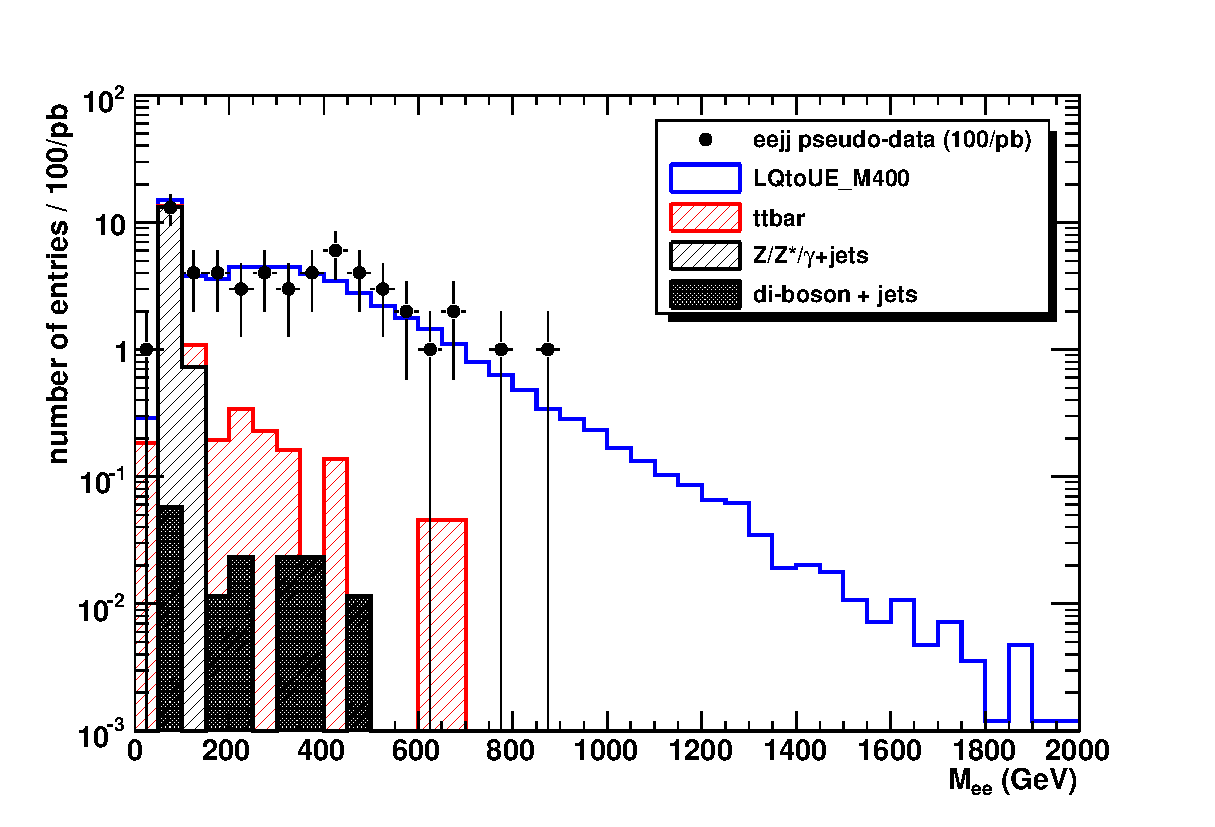
\includegraphics{plots/LQ400FullSimeejjFinalPlots/Mee_eejj_LQ400_100pb.eps}} &
      \resizebox{7.5cm}{!}{b)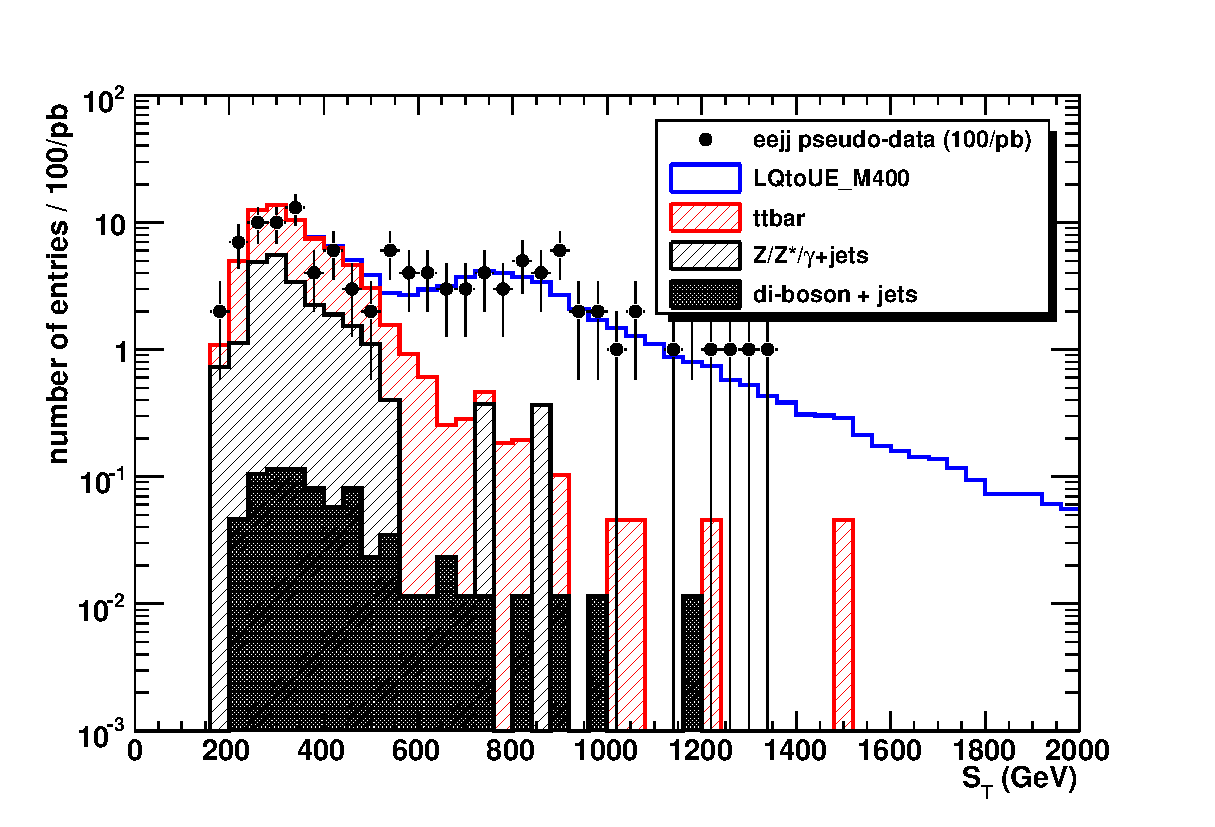
\includegraphics{plots/LQ400FullSimeejjFinalPlots/ST_eejj_LQ400_100pb.eps}} \\
    \end{tabular}
    \caption{\small \sl a) invariant mass of the electron pair, $M_{ee}$. \newline b) Scalar sum of the $P_T$ of the 2 leading electrons and 2 leading jets. 
	     In each histogram, the distributions for the signal with $M_{LQ}=400~$GeV 
	     and the contributing backgrounds 
	     (with the exception of the QCD background, see Section~\ref{sec:QCDBackground}) are shown after 
	     applying all cuts except the one involving the plotted variable. 
	    The histograms are cummulative.
	     }
    \label{fig:Mee_St_distributions}
  \end{center}
\end{figure}


\begin{figure}[htbp]
  \begin{center}
    \begin{tabular}{cc}
      \resizebox{7.5cm}{!}{a) 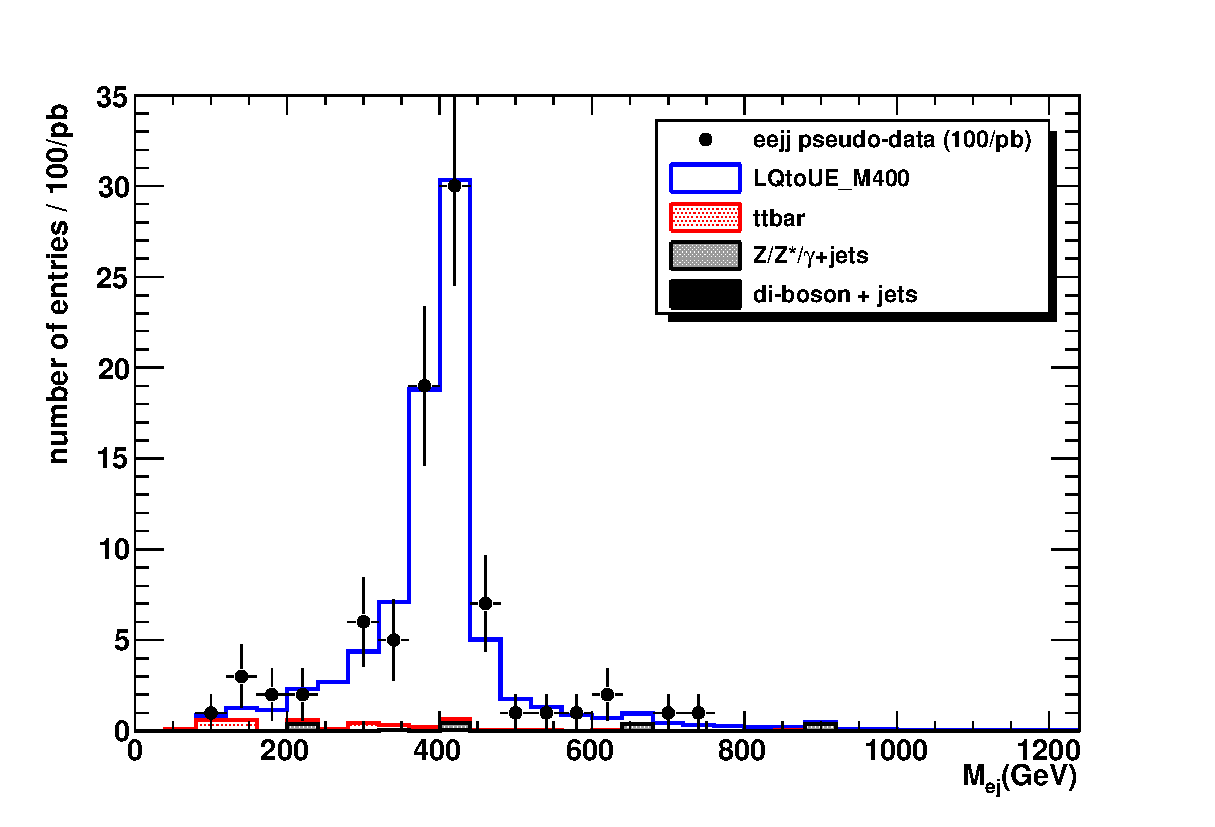
\includegraphics{plots/LQ400FullSimeejjFinalPlots/Mej_eejj_LQ400_100pb_LinScale.eps}} & 
      \resizebox{7.5cm}{!}{b) 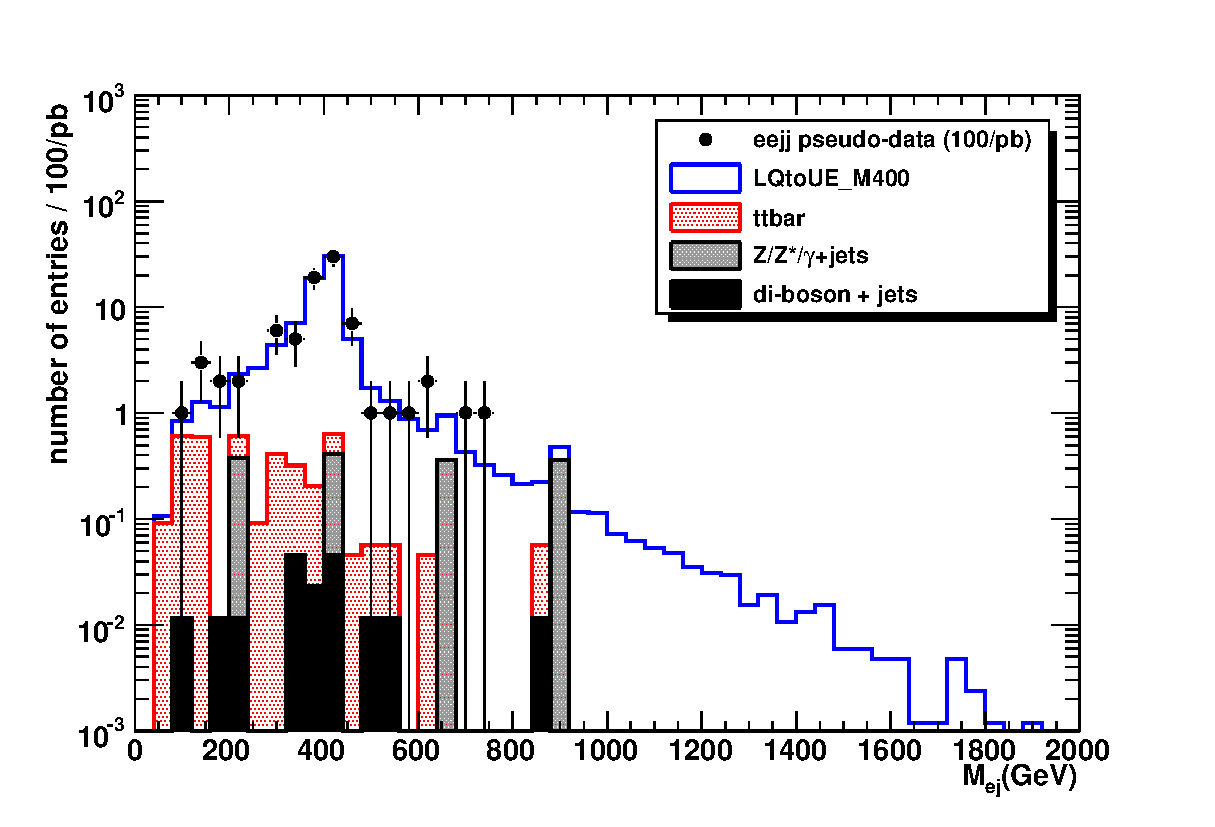
\includegraphics{plots/LQ400FullSimeejjFinalPlots/Mej_eejj_LQ400_100pb.eps}} \\
    \end{tabular}
    \caption{\small \sl Distribution of the invariant mass, $M_{ej}$, 
      of the electron-jet pairing with smaller $\Delta M_{ej}$, for signal with $M_{LQ}=400~$GeV and the contributing backgrounds 
      (with the exception of the QCD background, see Section~\ref{sec:QCDBackground}). 
      The complete event selection has been applied.
      All histograms are cummulative.
      The plot is shown in linear and log scale in a) and b) respectively. 
      }
    \label{fig:Mej_allComb}
  \end{center}
\end{figure}


The efficiency of each selection cut is shown in Table \ref{tab:effic-MLQ400} 
for a LQ sample with a mass of 400 GeV. 


\begin{table}[htbp] 
\begin{center} 
\begin{tabular}{|c|c|c|c|} 
\hline\hline 
 Cut & $N_{evt}$ passed for $100pb^{-1}$ & $\varepsilon_{rel}$ & $\varepsilon_{abs}$ \\ 
\hline\hline 
None       &        7.50e+01       $~\pm~$       0.00e+00        &        1.0e+00       $~\pm~$       0.0e+00        &        1.0e+00       $~\pm~$       0.0e+00       \\       
       Skim       &        6.80e+01       $~\pm~$       9.00e-02        &        9.1e-01       $~\pm~$       1.3e-03        &        9.1e-01       $~\pm~$       1.2e-03       \\       
       2 ele $P_T>30~$GeV       &        6.68e+01       $~\pm~$       9.00e-02        &        9.8e-01       $~\pm~$       1.9e-03        &        8.9e-01       $~\pm~$       1.2e-03       \\       
       2 ele (ID+Iso) $P_T>30~$GeV       &        5.01e+01       $~\pm~$       1.40e-01        &        7.5e-01       $~\pm~$       3.1e-03        &        6.7e-01       $~\pm~$       1.9e-03       \\       
       2 jets (Cleaned),$P_T>$50~GeV,$|\eta|<$3       &        4.69e+01       $~\pm~$       1.40e-01        &        9.4e-01       $~\pm~$       4.1e-03        &        6.3e-01       $~\pm~$       1.9e-03       \\       
       $M_{ee}>$100~GeV       &        4.49e+01       $~\pm~$       1.50e-01        &        9.6e-01       $~\pm~$       4.5e-03        &        6.0e-01       $~\pm~$       1.9e-03       \\       
       $S_T>$620~GeV       &        3.90e+01       $~\pm~$       1.50e-01        &        8.7e-01       $~\pm~$       5.1e-03        &        5.2e-01       $~\pm~$       2.0e-03       \\       
          \hline\hline 
\end{tabular} 
\end{center} 
\caption{Sample of $M_{LQ}=400~$GeV (FullSim): Sequence of selection cuts with number of events selected in 100$~pb^{-1}$, efficiency relative to the preceding cut and absolute efficiency. The reported uncertainties on the number of events and efficiencies are statistical, due to the number of analyzed MC events.} 
\label{tab:effic-MLQ400} 
\end{table} 



 
Table~\ref{tab:selection_effic_ttbar} shows the number of events selected by each cut 
for $t\bar{t}$ and $Z/\gamma$+jet events, which are the dominant backgrounds in the final sample. 
A summary of the number of selected signal and background events expected in 100 pb$^{-1}$ of data 
is reported in Table \ref{tab:EventSelSummary}. 
The overall signal selection efficiencys is around 3
5-65\% for the LQ masses investigated. 


\begin{table}[htbp]
\begin{center}
\begin{tabular}{|c| |c|c|}
\hline
\hline
 & $t\bar{t}$ sample  & $Z/\gamma$ sample\\
 & $N_{ev}$ $100pb^{-1}$ & $N_{ev}$ $100pb^{-1}$ \\
  
\hline
\hline
None       &        4.14e+04       $~\pm~$       0.00e+00  &        4.22e+05       $~\pm~$       0.00e+00           \\       
Skim       &        6.75e+03       $~\pm~$       1.61e+01 &        9.01e+03       $~\pm~$       5.67e+01       \\       
2 ele $P_T>30~$GeV &        1.75e+03       $~\pm~$       8.77e+00&        2.65e+03       $~\pm~$       3.10e+01     \\       
2 ele (ID+Iso) $P_T>30~$GeV &        1.55e+02       $~\pm~$       2.66e+00 &        2.02e+03       $~\pm~$       2.70e+01     \\       
2 jets (Cleaned),$P_T>$50~GeV,$|\eta|<$3 &        7.72e+01       $~\pm~$       1.88e+00 &        3.28e+02       $~\pm~$       1.09e+01        \\       
$M_{ee}>$100~GeV &        4.62e+01       $~\pm~$       1.45e+00 &        2.29e+01       $~\pm~$       2.89e+00        \\       
$S_T>$620~GeV &        1.46e+00       $~\pm~$       2.60e-01 &        7.30e-01  $~\pm~$       5.20e-01        \\       
\hline
\end{tabular}
\end{center}
\caption{\small \sl $t\bar{t}$ and $Z/\gamma$ samples: the first column lists the selection sequence. ``$N_{ev}$  $100pb^{-1}$'' is the number of selected events in $100pb^{-1}$.}
\label{tab:selection_effic_ttbar}
\end{table}


\begin{table}[htbp]
\begin{center}
\begin{tabular}{|lcc||cccc|}
\hline\hline
Signal Samples       & $S_T$ cut       & Number of Events     & Number              & of Events           & in Background    & Samples     \\
                     & (GeV)           & in Signal Samples    & $t\bar{t}$ + N jets & $Z/\gamma$ + N jets & QCD              & VV + N jets \\ 
\hline
$M_{LQ}=250~$GeV     & 460             & 342.06 $\pm$ 2.10    & 7.18  $\pm$ 0.57    & 2.55  $\pm$ 0.96    & 0.37 $\pm$ 0.37  & 0.21 $\pm$ 0.05 \\ 
$M_{LQ}=250~$GeV (*) & 460             & 359.39 $\pm$ 1.36    & as above            & as above            & as above         & as above        \\
$M_{LQ}=300~$GeV (*) & 520             & 163.37 $\pm$ 0.53    & 3.89  $\pm$ 0.42    & 1.09  $\pm$ 0.63    & 0.37 $\pm$ 0.37  & 0.15 $\pm$ 0.04 \\ 
$M_{LQ}=400~$GeV     & 620             &  38.98 $\pm$ 0.15    & 1.46  $\pm$ 0.26    & 0.73  $\pm$ 0.52    & 0.37 $\pm$ 0.37  & 0.09 $\pm$ 0.03 \\ 
$M_{LQ}=400~$GeV (*) & 620             &  40.41 $\pm$ 0.10    & as above            & as above            & as above         & as above        \\
$M_{LQ}=500~$GeV (*) & 740             &  11.56 $\pm$ 0.03    & 0.69  $\pm$ 0.18    & 0.36  $\pm$ 0.36    & 0.00 $\pm$ 0.00  & 0.05 $\pm$ 0.02 \\ 
$M_{LQ}=600~$GeV (*) & 740             &   4.04 $\pm$ 0.01    & as above            & as above            & as above         & as above        \\
%$M_{LQ}=650~$GeV (*) & 740             &   2.43 $\pm$ 0.01    & as above            & as above            & as above         & as above        \\
%$M_{LQ}=700~$GeV (*) & 740             &   1.49 $\pm$ 0.00    & as above            & as above            & as above         & as above        \\
%$M_{LQ}=800~$GeV (*) & 740             &   0.59 $\pm$ 0.00    & as above            & as above            & as above         & as above        \\
%$M_{LQ}=900~$GeV (*) & 740             &   0.25 $\pm$ 0.00    & as above            & as above            & as above         & as above        \\
%$M_{LQ}=1000~$GeV (*)& 740             &   0.11 $\pm$ 0.00    & as above            & as above            & as above         & as above        \\
\hline\hline
\end{tabular}
\end{center}
\caption{\small \sl Number events expected from LQ signal and background samples after the analysis selection for 100 pb$^{-1}$ of data.
The cut value on the kinematic variable $S_T$ depends on the LQ mass, and it is indicated in the second column.
Data samples from FullSim Monte Carlo are used for all backgrounds and for LQ masses of 250 and 400 GeV. 
Signal samples marked by (*) are made with the FastSim Monte Carlo. } 
\label{tab:EventSelSummary}
\end{table}

\subsection{Cut Optimization} \label{sec:cutOptimization}

Eight variables are studied to optimize the selection of  events,
 the $p_T$'s of the two leading electrons and two leading jets, the 
restriction 
on $\eta$ for the electrons, the restriction on 
$\eta$ for jets, the invariant mass $M_{ee}$ of the two leading electrons, 
and  $S_T$.
The result of the optimization for LQ's with mass of 250 GeV for
the requirement on $|\eta^{ele}|$ prefers as large a value as possible
(2.5, the acceptance of the tracker)
and $|\eta^{jets}|<3$. 
The cut on the invariant mass of the two electrons 
is optimal at  $M_{ee}>100$ GeV. The 
optimal cut values for electron and jet $p_T$ are consistently 
the lowest considered value in the scanned range 
(20 GeV). However, the $p_{T}$ cut on electrons is increased to 
30 GeV since the rate for jets faking electrons will have
large uncertainties at startup~\cite{HEEPNOTE}; 
%FIXME%
the $p_{T}$ cut on jets is increased to 50 GeV in order to reduce the effect 
of uncertainties in the initial and final state radiation, and the uncertainties 
on calorimeter response at the start-up (not considered during the
optimization procedure).
These changes have a negligible effect on the signal significance. 
This optimization indicates the $S_T$ cut 
should increase with LQ mass. 
The optimized values of $S_{T}$ cuts for different mass hypotheses are shown in Table~\ref{tab:EventSelSummary}. 


\section{Data-driven techniques for background estimate} \label{sec:bkgStudy}
After the event selection the dominant number of SM backgrounds 
 come from $t\bar{t}$ and $Z/\gamma$+jet processes, 
as summarized in table \ref{tab:EventSelSummary}. 
Sections~\ref{sec:ttbarControlSample} and~\ref{sec:ZcontrolSample} 
describe data-driven techniques that use control samples 
to estimate the absolute 
normalization for these two backgrounds, and the shapes of the distributions of
the selection variables 
for the $t\bar{t}$ background. 

\subsection{$t\bar{t}$ background control sample} \label{sec:ttbarControlSample}
A useful control sample can be obtained by 
requiring at least one electron and one muon, instead of at least 2 electrons, 
in the final state, in addition to the two jets. 
For $t\bar{t}$ events, the distributions for the selection variables
for the e$\mu$jj and the eejj samples
are expected to be very similar in shape, since the kinematics 
of the process do not depend 
on the nature of the lepton. 
Figure~\ref{fig:ttbar} shows good agreement between 
the shape of $M_{lj}$ and $S_{T}$ distributions 
with the current MC statistics available. Similar agreement 
is found for the other reconstructed kinematic variables 
used in the selection. 

\begin{figure}[htb]
  \begin{center}
  \begin{tabular}{cc}
  \resizebox{8cm}{!}{a) 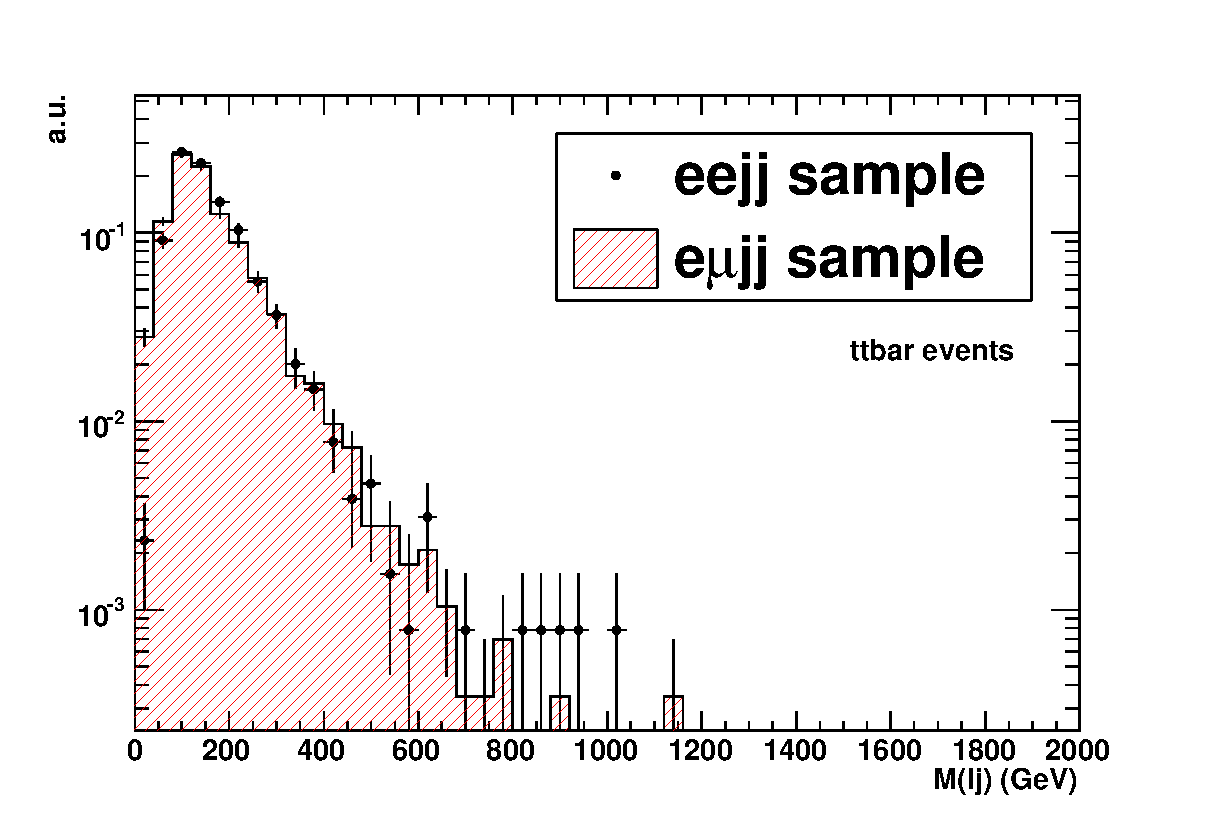
\includegraphics{plots/ttbarStudies/Mlj_eejj_VS_emujj_ttbar_STcut300.eps}} &
  \resizebox{8cm}{!}{b) 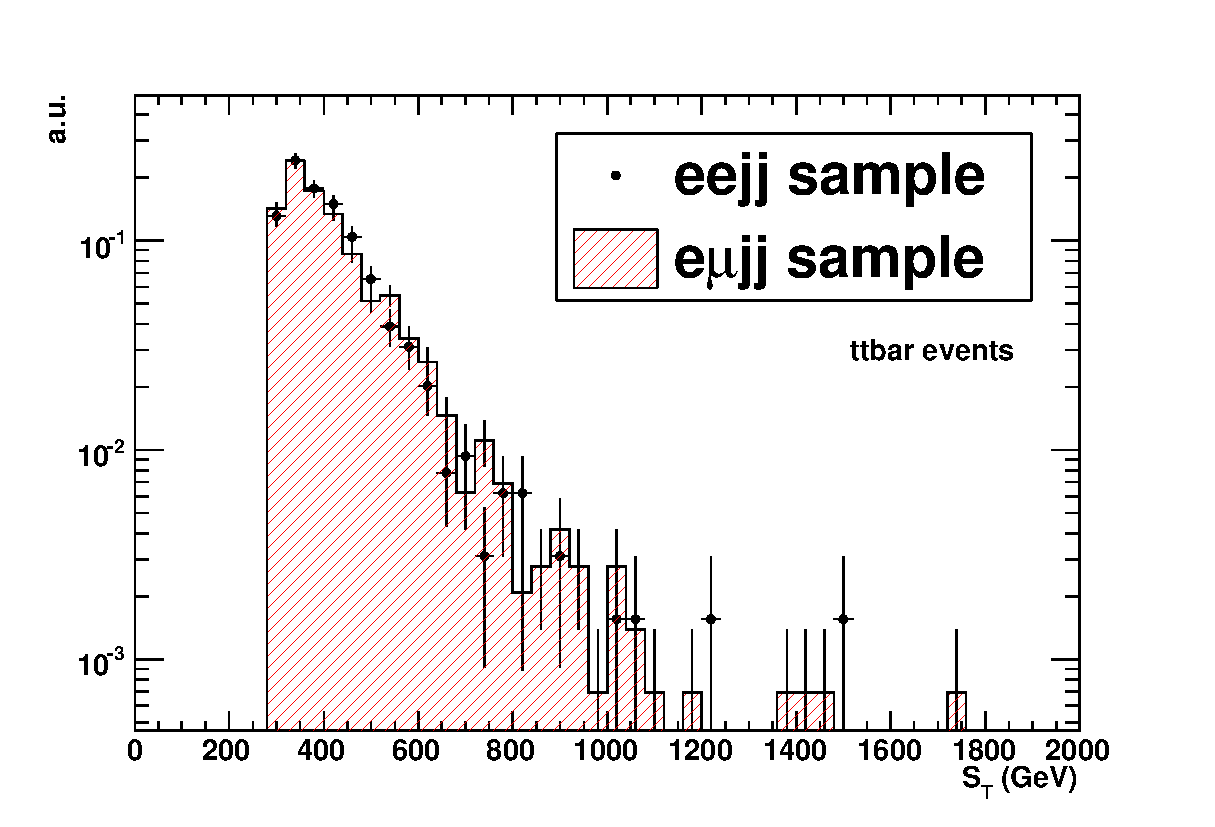
\includegraphics{plots/ttbarStudies/ST_eejj_VS_emujj_ttbar_STcut300.eps}} \\
  \end{tabular}
  \caption{\small \sl Distributions of the lepton-jet invariant mass (a) and $S_{T}$ (b) for the eejj and the e$\mu$jj samples, for $t\bar{t}$ events.
  All baseline selection criteria  
  described in Section~\ref{sec:eventSelection} are applied with
the $S_{T}$ cut set to 300 GeV.}
  \label{fig:ttbar}
  \end{center}
\end{figure}

The e$\mu$jj sample is dominated by $t\bar{t}$ events, 
with a small contamination estimated from MC of less than 5\% (for an 
$S_{T}$ cut of 300 GeV), 
mainly from di-boson events. (For $W$+jets and $Z/\gamma$+jets 
contributions, the statistical 
uncertainties are large, around 100\%, due to limited MC statistics.) 
For $t\bar{t}$ events, the e$\mu$jj sample with 100 pb$^{-1}$ of data 
is expected to have about 66, 11, and 5 events, respectively, 
for $S_{T}$ cuts of 300, 520 (used for LQ's with a mass of
300 GeV), and 620 GeV (used for LQ masses of 400 GeV).

Although the W decays with equal branching fraction to electrons and muons,
the trigger filter, the offline selection, and the 
different reconstruction efficiencies,
acceptances, and $P_{T}$ resolutions  bias the number of selected eejj 
and e$\mu$jj events. 
In this analysis, we correct for the different reconstruction efficiencies
(which is the dominant effect for the current selection) by
binning the events in the $P_T$ of the leading lepton and using

\begin{equation} \label{formula:NeejFromNemujj}
N_{eejj}^{est.} = \frac{1}{2}\sum_{P_{T}^{\mu}} N_{e\mu jj}(P_{T}^{\mu}) \times R(P_{T}^{\mu}) \quad , 
\end{equation}

where $N_{e\mu jj}(P_{T}^{\mu})$ is number of events in the bin, 
and $R(P_{T})$ is the ratio between electron 
and muon reconstruction efficiencies as a function of lepton $P_{T}$. 
The ratio $R(P_{T})$ was obtained 
using a MC FullSim sample of Z+jets 
events with an equivalent integrated luminosity of 275 $pb^{-1}$.
The value of $R(P_{T})$ is between 0.85-0.95 for $30 < P_{T} < 500$ GeV.
Once real data becomes available this ratio could be obtained with $tag\&probe$ method using $Z \rightarrow ee$ and 
$Z \rightarrow \mu\mu$ events.

\subsection{$Z/\gamma$+jet background control sample} \label{sec:ZcontrolSample}

A control sample that can be used to
estimate the $Z/\gamma$+jet background (eejjAtZ sample) 
can be obtained by using the full selection criteria except reversing 
the $M_{ee}$ cut to select events consistent with a $Z$ boson
($80\mbox{ GeV} < M_{ee} < 100\mbox{ GeV}$). 
This control sample is an almost pure sample of  
$Z/\gamma$+jet events 
( less than 4\% contamination, dominated by $t\bar{t}$ events, 
for an $S_{T}$ cut of 300 GeV). 
%the eejjAtZ sample is independent from the eejj signal sample by construction. 
The eejjAtZ sample with 100 pb$^{-1}$ of data 
is expected to have about 129, 22, and 12 events, respectively for an $S_{T}$ cut of 300, 520, and 620 GeV.

%\begin{figure}[htb]
%  \begin{center}
%  \begin{tabular}{cc}
%  \resizebox{10cm}{!}{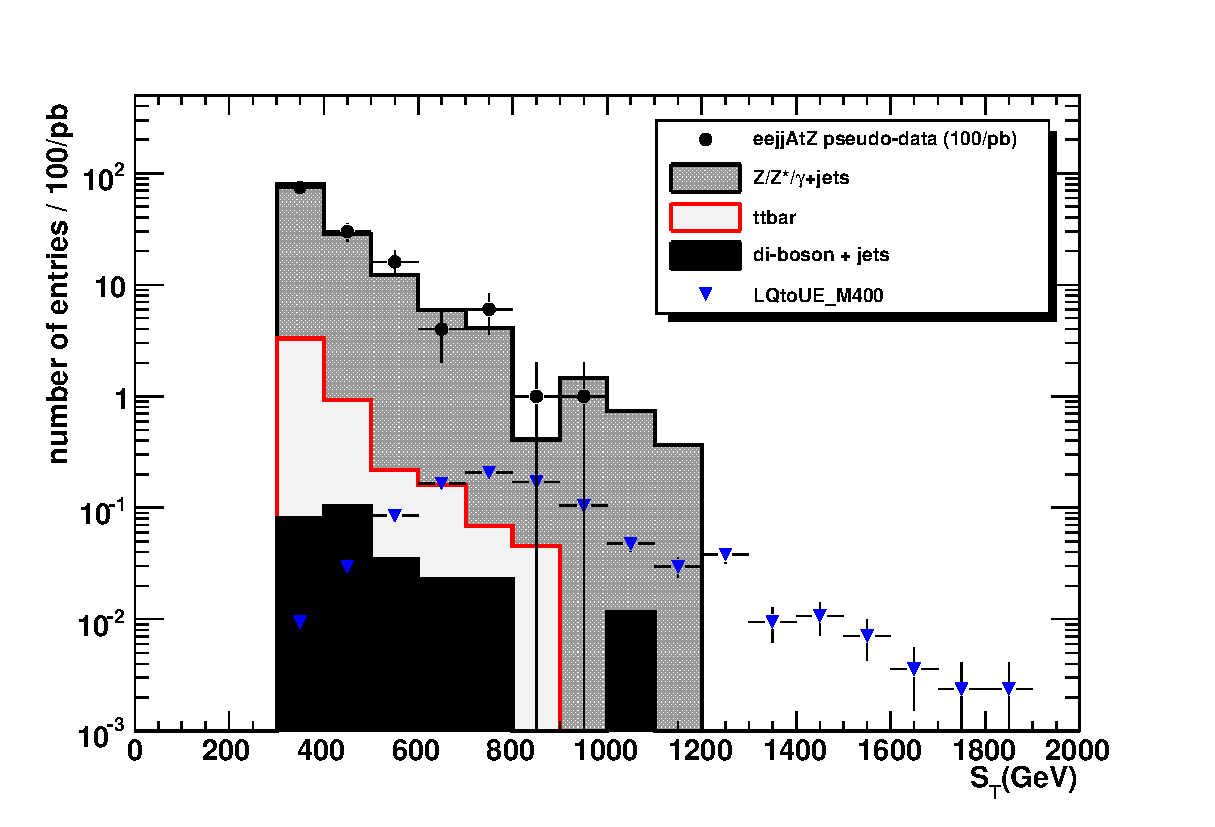
\includegraphics{plots/ZjetStudies/ST_100InVpb_eejjAtZ_looseSTcut_MeeInverted_WithLQ400.eps}} \\ 
%  \end{tabular}
%%  \caption{\small \sl Distribution of the $P_{T}$ at generator level of the electron pair ($P_{T}$ of the boson) 
%%    for $Z/\gamma$+jet events in the signal eejj sample 
%%    (cut 1,2,3,4)
%%    and the control sample (cut 1,2,4 + $80\mbox{ GeV} < M_{ee} < 100\mbox{ GeV}$), for $Z/\gamma$+jet events.}
%  \caption{\small \sl Distribution of the $S_{T}$ variable for eejjAtZ sample
%    for different background components. 
%    Histogram of signal events (at 400~GeV LQ mass) is also added. 
%    Baseline selection criteria (cut 1,2) described in Section~\ref{sec:eventSelection} 
%    are applied, $S_{T}$ cut has been set to 300 GeV, 
%    cut on $M_{ee}$ is modified to select real Z bosons ($80\mbox{ GeV} < M_{ee} < 100\mbox{ GeV}$).
%    The background histograms are summed on top of each other.
%    Black dots indicate pseudo data randomly generated accordingly with 
%    the total background distribution, and assuming 100 $pb^{-1}$ of data.}
%  \label{fig:eejjAtZContamination}
%  \end{center}
%\end{figure}
%
The background in the final sample is estimated by
rescaling the control sample using a 
hybrid method which combines the eejjAtZ data with 
MC information.  
The number of $Z/\gamma$+jet events in 
the eejj signal sample ($M_{ee}>100$ GeV) can be estimated by

\begin{equation} \label{formula:NeejFromRoffZatZ}
N_{eejj}^{Z} = N_{eejjAtZ} \times R_{OffZ/AtZ} \quad , 
\end{equation}

where $N_{eejjAtZ}$ is the number of events in the eejjAtZ control sample, and 
$R_{OffZ/AtZ}$ is the ratio between the number of $Z/\gamma$+jet events 
with $M_{ee} > 100\mbox{ GeV}$ (OffZ events) and $80\mbox{ GeV} < M_{ee} < 100\mbox{ GeV}$ 
(AtZ events) that have passed all the other selection criteria.
In this analysis the value of $R_{OffZ/AtZ}$ is determined directly from MC.
%The motivations that justify this approach are discussed below:
%%
%\begin{itemize}
%%
%\item Those theoretical uncertainties that are independent 
%on the value of two electron invariant mass cancel in the ratio.
%\item For inclusive Drell-Yan production ($Z/\gamma \rightarrow ee$ with no jets), 
%the MC is expected to predict the value of this ratio with small 
%uncertainty (dominated by PDF uncertainties). 
%The data-MC comparison will be done with real data by calculating 
%the ratio $R_{OffZ/AtZ}$ using a control sample with only two electrons 
%(which is expected to be dominated by Drell-Yan events 
%up to values of $M_{ee}$ of several TeV~\cite{HEEPNOTE}).
%\item The next step will be to compare the distributions of reconstructed selection 
%variables between eejjAtZ data and MC to check the agreement in the control region.
%It is expected to have more confidence in the MC extrapolation 
%from the control region to the signal region (i.e. the estimation of the ratio $R_{OffZ/AtZ}$), 
%if the event kinematics in the two regions is not dramatically different.
%Figure~\ref{fig:STEleJetceejjAtZvsOffZ}
%show the distributions of the scalar sum of $P_{T}$ of the two leading electrons ($S_{T}^{ele}$) 
%and the two leading jets ($S_{T}^{jets}$) for $Z/\gamma$+jet events, 
%in both signal region (eejj sample) and control region (eejjAtZ control sample). 
%A significant discrepancy is observed 
%in the $S_{T}^{ele}$ distribution; this should not represent 
%a problem for the MC extrapolation, since the Electro-Weak part of the process 
%is well predicted, and the expected agreement could be directly checked with a control sample 
%of two electrons (as described in the previous bullet).
%It's also comforting that the $S_{T}^{jet}$ distributions are not dramatically different, 
%which is an indication that the hadronic part of the $Z/\gamma$+jet process 
%(the one with largest uncertainties) is similar between 
%signal and control region.  
%%
%\end{itemize}
%
%\begin{figure}[htb]
%  \begin{center}
%  \begin{tabular}{cc}
%    a.
%    \resizebox{8cm}{!}{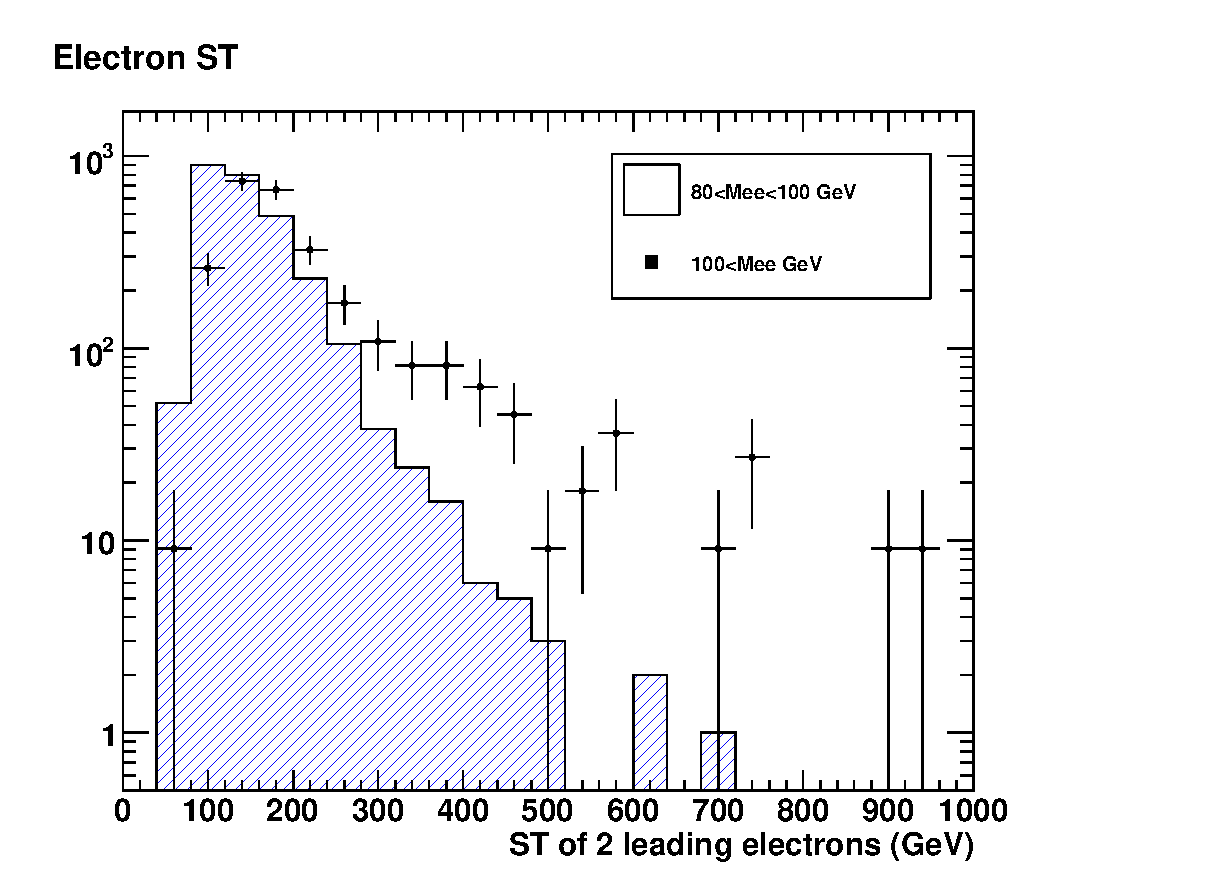
\includegraphics{plots/ZjetStudies/ST_Elecs_inside.eps}} &
%    b.
%    \resizebox{8cm}{!}{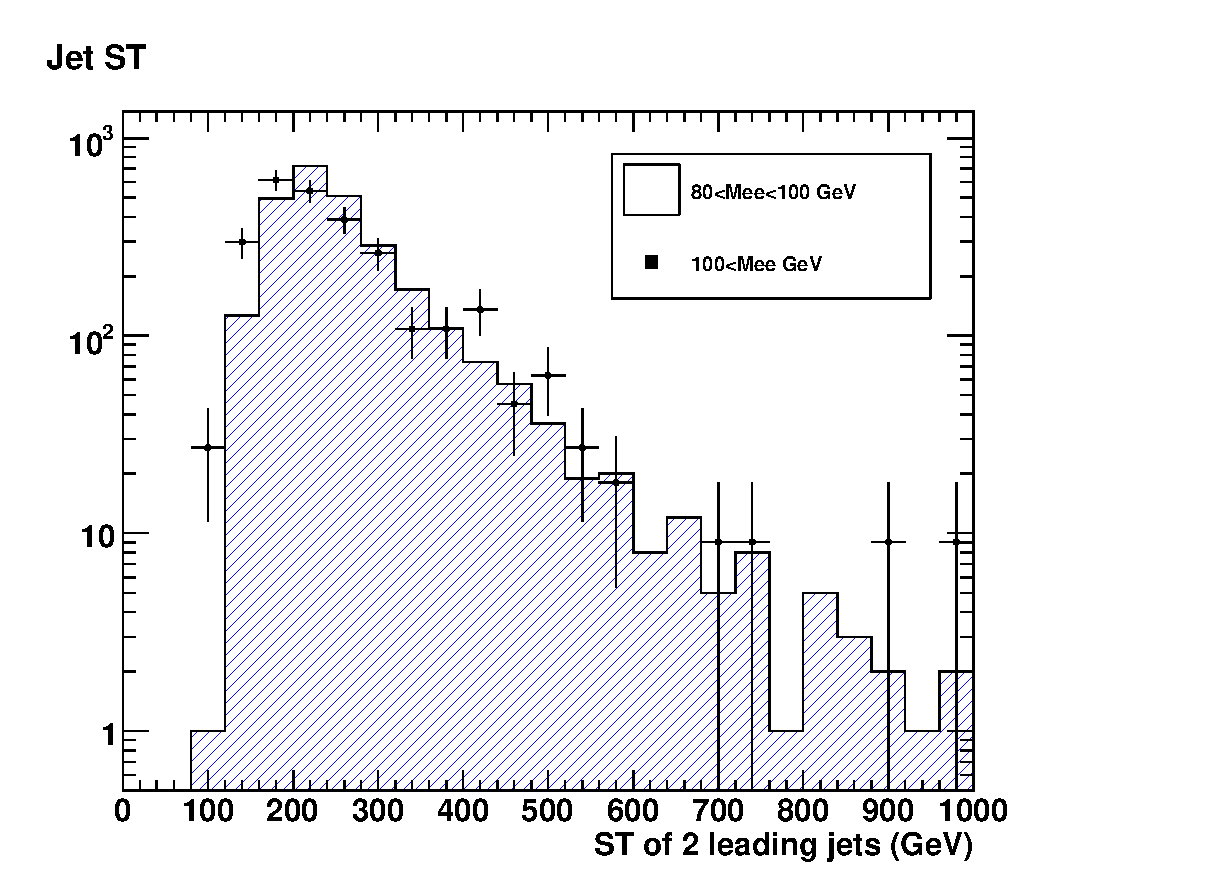
\includegraphics{plots/ZjetStudies/ST_Jets_inside.eps}} \\
%  \end{tabular}
%  \caption{\small \sl Distributions of (a) $S_{T}^{ele}$ (b) $S_{T}^{jet}$ 
%    for the signal eejj sample ($M_{ee} > 100\mbox{ GeV}$) 
%    and the eejjAtZ control sample ($80\mbox{ GeV} < M_{ee} < 100\mbox{ GeV}$), 
%    using a large FastSim sample of $Z/\gamma$+jet events.}
%  \label{fig:STEleJetceejjAtZvsOffZ}
%  \end{center}
%\end{figure}
%
%

\subsection{QCD Background} \label{sec:QCDBackground}

The MC statistics of the QCD sample is not sufficient to perform a reasonable estimate of the contamination 
of QCD events in the eejj sample, although it seems to confirm the expectation that it is small compared with 
the dominant $t\bar{t}$ and $Z/\gamma$+jet backgrounds (see Table~\ref{tab:EventSelSummary}). 
In addition, large uncertainties are expected on the cross section of QCD production at LHC start-up.
For this reason different techniques (possibly data-driven) are preferred to estimate the QCD background.

The simple approach used in this analysis is to take a QCD sample with two fake electrons and two jets (ffjj sample)
that pass all the kinematic selection criteria (see Section~\ref{sec:eventSelection}), and rescale it to estimate 
the QCD contamination in the eejj sample as
%
\begin{equation} \label{QCDRescaling}
N_{eejj}^{QCD} = N_{ffjj}^{QCD} \times {P(e|f)}^2 \quad , 
\end{equation}
%

where ``f'' is a reconstructed electron with loose ID requirements (all objects in the initial electron collection 
before applying HEEP ID and Isolation), 
``e'' is a reconstructed electron which pass all the HEEP ID and Isolation criteria (see Table~\ref{tab:HEEPselection} 
of Section~\ref{sec:electrons}), 
$N_{eejj}^{QCD}$ ($N_{ffjj}^{QCD}$) is the number of QCD events in the eejj (ffjj) sample (control sample), 
and $P(e|f)$ is the probability of a fake electron (f) to pass the HEEP ID and Isolation requirements (e).
The probability $P(e|f)$ is obtained from the rate of ``f'' to ``e'' in a ffjj sample of QCD events 
(QCD ($H_T\in[500,1000]$~GeV) is used since it's the largest contribution in the control sample) .
The number of QCD events in the eejj and ffjj sample are calculated using 
an $S_{T}$ cut of 460 GeV (which is the optimized cut for LQ mass of 250 GeV), and assuming 100 $pb^{-1}$ of data.

The probability $P(e|f)$ is found to be $\approx 2 \cdot 10^{-3}$, almost flat in the barrel region ($|\eta|<1.5$), while 
it is increasing with $\eta$ in the endcap region, up to $\approx 2 \cdot 10^{-2}$ for $|\eta|=2.5$. 
The average value $P(e|f) = 3.5 \cdot 10^{-3}$ is used.
The value of $N_{ffjj}^{QCD}$ is found to be $6130 \pm 47$. The number of QCD events in the eejj sample is estimated 
by rescaling the ffjj sample with Equation~\ref{QCDRescaling}, and it is $N_{eejj}^{QCD}=0.075$ events.
This value is in agreement with the estimate of $0.37 \pm 0.37$ events 
(see Table~\ref{tab:EventSelSummary}) obtained by directly applying the full eejj 
selection on the QCD MC sample. An uncertainty of 200\% on the value of $P(e|f)$ is estimated 
from closure tests performed with relaxed ID and Isolation cuts. 

\section{Systematic Uncertainties} \label{sec:Systematics}

The main sources of systematic uncertainties for this analysis are discussed below.

%
\begin{enumerate}
\item Uncertainty in the jet and electron energy scale

To quantify the effect of the uncertainty on the reconstructed energy of the electron and jets,
the analysis is repeated rescaling the electron and jet energies
 with a multiplicative factor. 
A variation of the jet energy of $\pm$10\% leads to a change of approximately 
7\% in the signal efficiency and 33\% in the number of background events, 
%(from $2.29 \pm 0.58$ to $3.04 \pm 0.61$ when the jet energy is {\sl increased} 10\%)
while a $\pm$5\% variation in the electron energy yields approximately a 3.5\% maximum 
change in signal efficiency and 35\% in the number of background events. 
%(from $2.29 \pm 0.58$ to $3.08 \pm 0.70$
%when the electron energy is {\sl increased} 10\%).  
%FIXME - rerun this for all mass points%
%
\item Uncertainty in the integrated luminosity of the data

This uncertainty is estimated to be 10\% for the first several months of LHC running~\cite{PTDR}. 
%
\item Statistical uncertainty on the MC data

The uncertainty on the final number of selected events for the FullSim sample with a leptoquark mass of 400 GeV is 
approximately 0.4\%.  The number of events produced 
for some of the background samples, however, correspond to a much
smaller equivalent integrated luminosity.  
The statistical uncertainty on the number of MC events is summarized for signal and background samples 
in table~\ref{tab:EventSelSummary} of Section~\ref{sec:eventSelection}.  
%
\item Uncertainties on FastSim selection efficiencies with respect to FullSim

The signal samples produced with FastSim show a slightly higher selection efficiency than FullSim, 
mostly due to the higher reconstruction efficiency of the electrons in the FastSim. 
This leads to a higher final selection efficiency in FastSim compared to FullSim by approximately 5\% 
for leptoquark samples with a mass of 250 and 400 GeV. FullSim samples at higher mass are not available 
to perform the comparison. A conservative uncertainty of 10\% on the selection efficiency 
for FastSim samples is used in the whole mass range investigated. 
%
\item Uncertainty from the data-driven background estimates

Estimates of the background by data-driven techniques are affected by the statistical
uncertainties on the size of the control samples.
The number of events expected in each control sample varies with the $S_T$ cut used, as 
described in section~\ref{sec:bkgStudy}. These uncertainties can be correctly estimated 
only when data is available, and they are not included in the discovery and exclusion potential
for this analysis.
%
\item Theoretical uncertainties 

At the LHC the PDF uncertainties are expected to give a non-neglible
contribution to the theoretical uncertainties using the
method developed by the CTEQ collaboration (cite cteq note)
The relative uncertainties on the differential cross sections 
typically range from 2-5\% for Standard Model processes, 
but may rise to 10\% or larger for parton processes at the TeV-scale 
(like the leptoquark pair production).
These uncertainties will be evaluated and included in future upgrades of this analysis.
\end{enumerate}



\section{CMS Discovery and Exclusion Potential} \label{CMSpotential}

In order to estimate the potential of the CMS detector to discover the first generation leptoquarks
in the electron channel, a simple counting experiment approach is used. 
The number of signal and background events expected for an integrated luminosity of
100~$pb^{-1}$ listed in Table~\ref{tab:EventSelSummary} and the systematic uncertainties described 
in Section~\ref{sec:Systematics} are used. 
The QCD background estimates from Table~\ref{tab:EventSelSummary} 
are not included because they are expected to be 
small compared to the other main background contributions (see Section~\ref{sec:QCDBackground}).
The effects of these systematic uncertainties are taken into account
by summing them in quadrature when calculating discovery and exclusion potential, unless otherwise noted.


To quantify the significance of the
leptoquark signal, the 
$S_\text{cP}$ significance estimator~\cite{ref:scp} is used.  
For a Poisson distribution
with mean $b$,
the probability to observe $n=s+b$ events or greater as:
\begin{equation}
P = p(n\geq s+b|b) = \sum_{n=s+b}^{+\infty} \frac{b^n}{n!}e^{-b},
\end{equation}
where $s$ and $b$ are the expected numbers of signal and background events, respectively. This probability can be
converted into an equivalent number of standard deviations using the one-sided Gaussian probability
\begin{equation}
P = \frac{1}{\sqrt{2\pi}}\int_{S_\text{cP}}^{+\infty} e^{-\frac{x^2}{2}}\mathrm{d}x,
\label{eq:ScP}
\end{equation}
which is the $S_\text{cP}$ significance.
Figure~\ref{fig:discovery}a. shows the required integrated luminosity
for a $5\sigma$ discovery for different leptoquark mass hypotheses. 

\begin{figure}[htb]
  \begin{center}
  \begin{tabular}{cc}
  \resizebox{8cm}{!}{a. 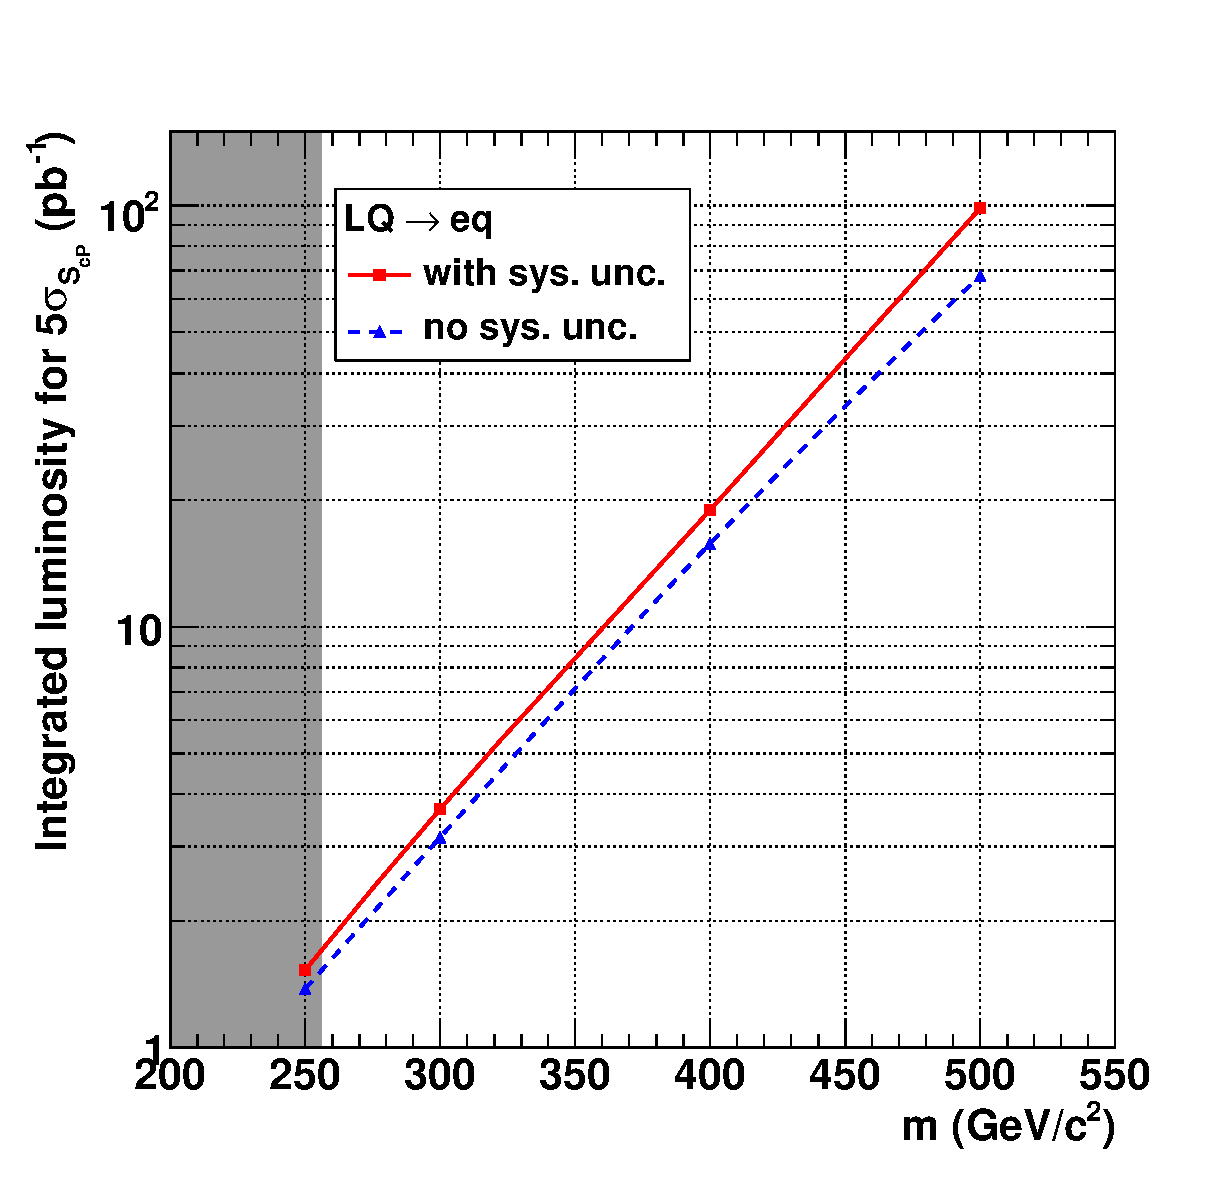
\includegraphics[width=0.5\textwidth]{plots/cmsPotential/L5sigma_vs_m_log.eps}}
  \resizebox{8cm}{!}{b. 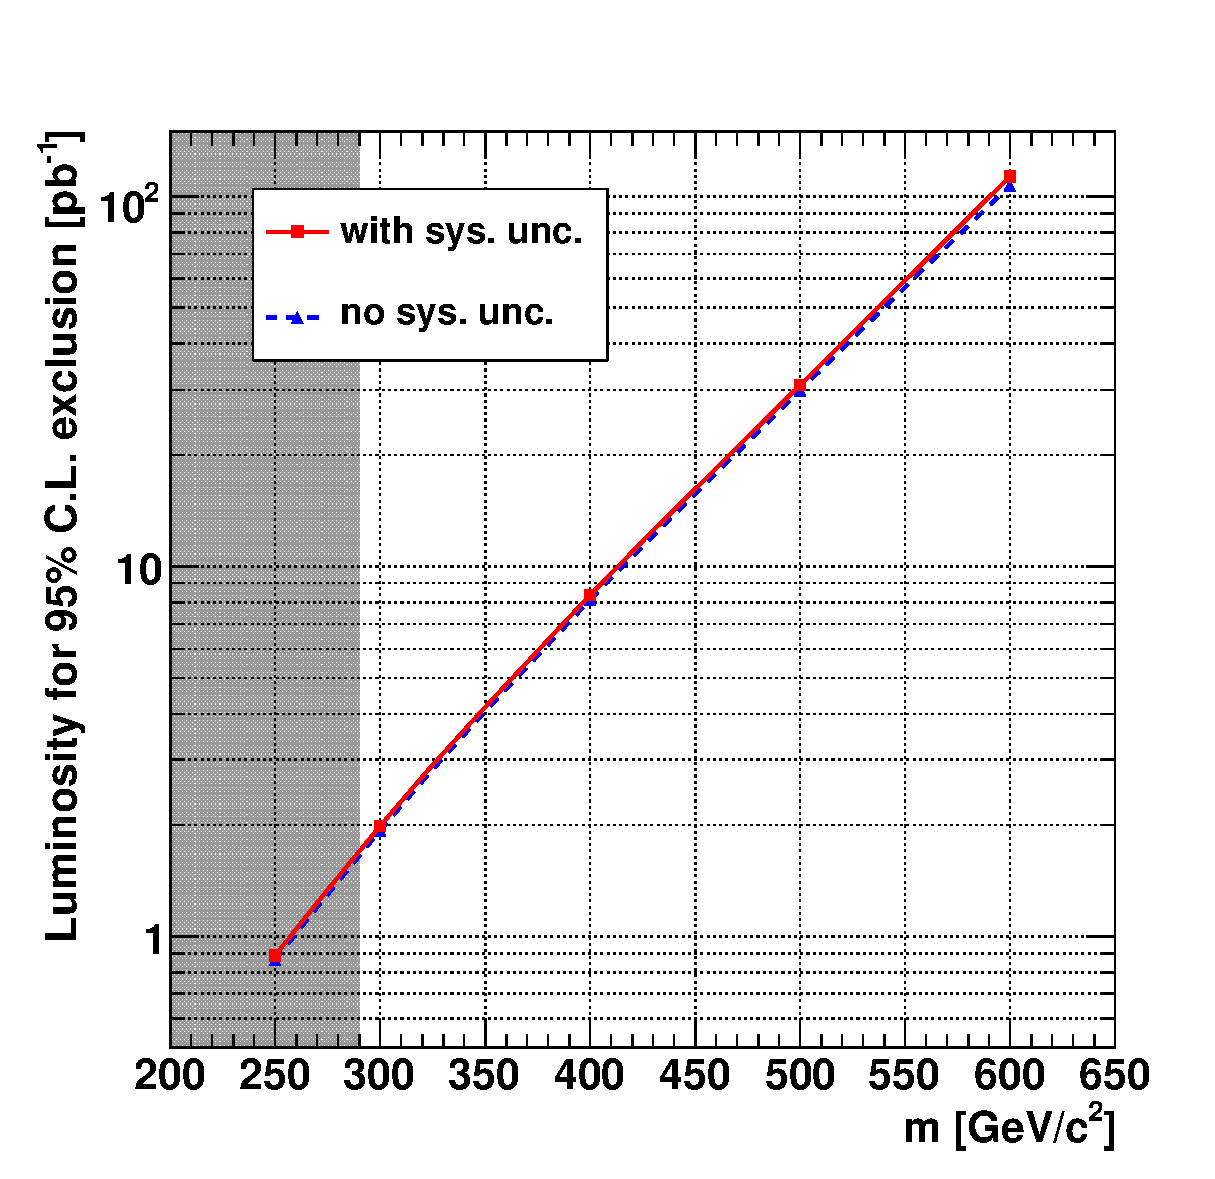
\includegraphics[width=0.5\textwidth]{plots/cmsPotential/L95CL_vs_m_log.eps}}
  \end{tabular}
 \caption{\small \sl a. Integrated luminosity
for a $5\sigma$ discovery for different leptoquark mass hypotheses assuming $\beta=1$. Solid red line includes the systematic uncertainties described in 
Section~\ref{sec:Systematics}. Shaded region is excluded by the current Tevatron limits.\newline
b. Integrated luminosity
for $95\%$ C.L. exclusion of different leptoquark mass hypotheses assuming $\beta=1$. Solid red line includes the systematic
uncertainties described in Section~\ref{sec:Systematics}. Shaded region is excluded by the current Tevatron limits.
}
 \label{fig:discovery}
  \end{center}
\end{figure}

For setting upper limits in the absence of the leptoquark signal, the Bayesian approach~\cite{ref:bayes} is used. 
Figure~\ref{fig:discovery} b. 
shows the required integrated luminosity for $95\%$ C.L. exclusion of different leptoquark mass hypotheses. 


\section{Conclusion}

The search for pair production of first generation leptoquarks that decay to
an electron and a jet is studied using a MC simulation.
The analysis strategy 
assume an integrated luminosity of 100 pb$^{-1}$ and $pp$ collisions 
at $\sqrt{s}=10$ TeV.
Standard CMS techniques are used for electron and jet identification. 
%Electron efficiencies will be determined from data using the Tag$\&$Pro [REF] technique. 
An optimized cut-based event selection has been applied.
The main expected background sources have been studied and two of them provide 
a significant contribution after event selection. 
Data-driven techniques to understand the characteristics of these contributions have been developed.

The discovery and exclusion potential in the channel with two electrons plus two jets has 
been determined using two statistical estimators suited for a counting experiment in the Poissonian regime.
The effect of the main systematic uncertainties 
has been studied and taken into account in the final 
results. This study has shown that, 
for leptoquark masses just above the Tevatron exclusion limit of 290~GeV
 assuming $\beta=1$, 
an early discovery is possible with a few $pb^{-1}$ of data.
With an integrated luminosity of 100~$pb^{-1}$, discovery should be possible up
to a leptoquark mass of 500, 400, and 250 GeV assuming, respectively, 
$\beta=1$, $0.5$, and $0.1$. 
In absence of evidence of a signal, the existence of a scalar leptoquark 
with mass lower than 600 GeV 
and $\beta=1$ can be excluded with 100~$pb^{-1}$ of data.


%--------------------------------------
%\clearpage
%--------------------------------------

\begin{thebibliography}{}

\bibitem {theories} {D.Acosta and S.K.Blessing, Ann.Rev.Nucl.Part.Sci 49,389},
  1999,
  {\em From June 2005}
\bibitem{hera}{H1 collaboration, Search for leptoquark bosons in ep collisions at HERA}, hep-ex/0506044,
\bibitem{d02008}{Search for First-Generation Leptoquarks in the dielectron channel with the DO Detector in $p\bar{p}$ Collisions at $\sqrt{s}=1.96$ TeV}, Jun 2008,
  {\em DO Note 5644-CONF}
\bibitem{cdf2005}{Search for first-generation scalar leptoquarks in $p\bar{p}$ collisions at $\sqrt{s}=1.96$ TeV}, Sept 2005,
  {\em Phys. Rev. D 72, 051107 (2005)} (CDF paper)
\bibitem{LQSingleAndPairProd}{Leptoquark Single and Pair production at LHC with CalcHEP/CompHEP in the complete model}, Feb 2005,
  {\em arXiv:hep-ph/0502067, JHEP0509:005,2005, MSU-HEP-070204}
  
  %  \bibitem{d02007}{Searches for LQ production at D0}, Oct 2007,
  %    {\em arXiv0710.0255v1}
  
  %\cite{Mangano:2002ea}
\bibitem{MADGRAPH}
  J. Alwall et Al.
  ``MadGraph/MadEvent v4: The New Web Generation''
  [arXiv:0706.2334].
  
  %  \bibitem{Mangano:2002ea}
  %    M.~L.~Mangano, M.~Moretti, F.~Piccinini, R.~Pittau and A.~D.~Polosa,
  %    ``ALPGEN, a generator for hard multiparton processes in hadronic collisions,''
  %    JHEP {\bf 0307} (2003) 001
  %    [arXiv:hep-ph/0206293].
  %    %%CITATION = JHEPA,0307,001;%%
  
\bibitem{HeepHlt}{D. Acosta et al., The CMS High Level Trigger}, CMS AN 2007/009,
\bibitem{Kramer}{M.Kramer et al., Pair production of scalar leptoquarks at the LHC},Jan 2008 ,{\em arXiv 0411038v2}
  %\cite{Abazov:2001mx} 	 
\bibitem{GSFele}{S. Baffioni et al., Electron Reconstruction in CMS}, CMS NOTE 2006/040,
\bibitem{HEEPNOTE} {CMS Collaboration, ``Search for high mass resonance production decaying into an electron pair in the CMS experiment''}, CMS PAS EXO-08-001
\bibitem{EleID}{D. Newbold et al., Electron ID at High Energies}, CMS AN 2008/045,
\bibitem{TagAndProbe}{CMS collaboration, Measuring Electron Efficiencies at CMS with Early Data}, CMS PAS EGM-07-001 (2007),
\bibitem{JetAlg} {P. Schieferdecker et al., Performance of Jet Algorithms in CMS}, CMS AN-2008/01,
\bibitem{Abazov:2001mx} 	 
  V.~M.~Abazov {\it et al.}  [D0 Collaboration], 	 
  %``Search for first-generation scalar and vector leptoquarks,'' 	 
  Phys.\ Rev.\  D {\bf 64} (2001) 092004 	 
  [arXiv:hep-ex/0105072]. 	 
  %%CITATION = PHRVA,D64,092004;%%
  %  \bibitem{highmassToMuons}{\bf I. Altsybeev et al., Search for new high-mass resonances decaying to muon pairs in the CMS experiment}, CMS AN 2007/038,
\bibitem{JES} {R. Harris, K. Kousouris, MC Truth L2 \& L3 Factorized Jet Corrections at CMS}, CMS AN-2008/03,
\bibitem{PTDR} {CMS Collaboration 2007, CMS Technical Design Report, Volum II: Physics Performance} 
J. Phys. G.: Nucl. Part. Phys. 34 995-1579, ``Luminosity Uncertainty'' at page 1500
\bibitem{PDFRescaling} {Parton Distribution Uncertainty Determination within CMSSW - CMS AN-2009/048}, FIXME
\bibitem{ref:scp} S. Bityukov, N. Krasnikov, S. Erofeeva, and A. Nikitenko, Program for evaluation of significance,
  confidence intervals and limits by direct calculation of probabilities, PhyStat 2005, Oxford, UK 
  [http://cmsdoc.cern.ch/~bityukov]
\bibitem{ref:bayes}  C. Amsler et al., Physics Letters B667, 1 (2008), section 32.3.1
  
\end{thebibliography}

\end{linenumbers}
\end{document}
